\documentclass[8pt]{beamer}

\newif\ifplacelogo % create a new conditional
\placelogotrue % set it to true

\usetheme{Warsaw}
\usecolortheme{rose}
\usepackage{multicol}
\usepackage{epstopdf}
\usepackage[italic]{hepnames}
\usepackage{tikz}
\usepackage{listings}
\usepackage{times}
\usepackage{amsmath}
\usepackage{verbatim}
\usepackage{hyperref}
\usepackage{bbding}
\usepackage{upgreek}
\usepackage{pdfpages}
\lstset{breakatwhitespace,
language=C++,
columns=fullflexible,
keepspaces,
breaklines,
tabsize=3, 
showstringspaces=false,
extendedchars=true}

% TikZ includes!!!
\usepackage{tikz}
\usetikzlibrary{backgrounds}
\usetikzlibrary{calc}
\tikzstyle{every picture}+=[remember picture]
\input{/home/oviazlo/Desktop/beamerPresentations/myReports/latexHelpScripts/tikzGrid.tex}


\begin{document}

% custom colors
\definecolor{olive}{rgb}{0.3, 0.4, .1}
\definecolor{fore}{RGB}{249,242,215}
\definecolor{back}{RGB}{51,51,51}
\definecolor{title}{RGB}{255,0,90}
\definecolor{dgreen}{rgb}{0.,0.6,0.}
\definecolor{gold}{rgb}{1.,0.84,0.}
\definecolor{JungleGreen}{cmyk}{0.99,0,0.52,0}
\definecolor{BlueGreen}{cmyk}{0.85,0,0.33,0}
\definecolor{RawSienna}{cmyk}{0,0.72,1,0.45}
\definecolor{Magenta}{cmyk}{0,1,0,0}

\definecolor{PixelColor}{RGB}{207,232,139}
\definecolor{SCTColor}{RGB}{167,166,255}
\definecolor{TRTColor}{RGB}{250,224,140}
\definecolor{grayColor}{RGB}{153,153,153}

\newcommand{\yRefPosOne}{0.0}
\newcommand{\xRefPosOne}{0.0}
\newcommand{\yRefPosTwo}{0.0}
\newcommand{\xRefPosTwo}{0.0}
\newcommand{\yRefIncrementOne}{0.0}
\newcommand{\xRefIncrementOne}{0.0}
\newcommand{\yRefIncrementTwo}{0.0}
\newcommand{\xRefIncrementTwo}{0.0}

\graphicspath{ {/home/oviazlo/Desktop/beamerPresentations/FCCee/pictures/may2_2018/} }


\DeclareGraphicsExtensions{.eps, .pdf, .png}

\newcommand{\myBox}[2][pink] {
    \noindent\colorbox{#1}{
	\textbf{#2}
    }\par
}

% For nice block (provided by Oleh)
\tikzstyle{myBox} = [draw=red, fill=blue!1, very thick,
    rectangle, rounded corners, inner sep=5pt, inner ysep=9pt]
    
\tikzstyle{PixelBox} = [draw=PixelColor, fill=blue!1, very thick,
    rectangle, rounded corners, inner sep=5pt, inner ysep=9pt]
\tikzstyle{SCTBox} = [draw=SCTColor, fill=blue!1, very thick,
    rectangle, rounded corners, inner sep=5pt, inner ysep=9pt]
\tikzstyle{TRTBox} = [draw=TRTColor, fill=blue!1, very thick,
    rectangle, rounded corners, inner sep=5pt, inner ysep=9pt]

% poster advertisement
\newcommand{\myCenterBox}[2][pink] {
   {\centering
    \noindent\colorbox{#1}{
	\textbf{#2}
    }\par
  }
}

\newcommand{\mySmallCenterBox}[2][pink] {
   {\centering
    \noindent\colorbox{#1}{
	\textbf{{\small #2}}
    }\par
  }
}

\newcommand{\myVerySmallCenterBox}[2][pink] {
   {\centering
    \noindent\colorbox{#1}{
	\textbf{{\scriptsize #2}}
    }\par
  }
}

\newcommand{\backupbegin}{
   \newcounter{finalframe}
   \setcounter{finalframe}{\value{framenumber}}
}
\newcommand{\backupend}{
   \setcounter{framenumber}{\value{finalframe}}
}

\newcommand{\myNode}{\tikz[baseline,inner sep=1pt] \node[anchor=base]}

\tikzstyle{fancytitle} =[fill=white!15, text=black]

\definecolor{light-gray}{gray}{0.95}
% poster advertisement


\title[ CLD detector performance  \hspace{16.5em}\insertframenumber/
\inserttotalframenumber]{ CLD detector model overview of layout and performances}


	\author[Oleksandr Viazlo]{Oleksandr Viazlo \\ 
% 	{\small ???}
	}
	\institute{\small CERN\\} 
	
       
	\date{10 April 2018}

% 	\logo{ \ifplacelogo \includegraphics[height=1.8cm]{./ID_week2/lund_uni-logo_s.pdf} \hspace{0.4cm} \fi}

	
%    	\frame{\titlepage}

   	

\placelogofalse

%*****************************************************************************
{
\setbeamercolor{background canvas}{bg=}
\includepdf[pages=1]{pg_0014.pdf}
}
%*****************************************************************************

%*****************************************************************************
\begin{frame}{\large \large Jet Energy Resolution}
\renewcommand{\yRefPosOne}{-0.5}
\renewcommand{\xRefPosOne}{4.2}
\renewcommand{\xRefIncrementOne}{7.5}
\begin{tikzpicture}[overlay]

 \node[inner sep=0pt] (tmp) at (\xRefPosOne-1.7,\yRefPosOne+0.9)
  {\includegraphics[width=6cm]{CLICbyMatthias_vs_FCCee_Zuds91.pdf}};
  
 \node[inner sep=0pt] (tmp) at (\xRefPosOne+4.5,\yRefPosOne+0.9)
{\includegraphics[width=6cm]{CLICbyMatthias_vs_FCCee_Zuds380.pdf}};

   \node  at (\xRefPosOne-3,\yRefPosOne+3) (box){%
    \myCenterBox{\small 91 GeV}
    };     
   \node  at (\xRefPosOne+3.2,\yRefPosOne+3) (box){%
    \myCenterBox{\small 380 GeV}
    };     
    
 \node  at (\xRefPosOne,\yRefPosOne-2.8) (box){%
    \begin{minipage}{0.9\textwidth}
      \begin{itemize}
		\item Comparabale performance at 91 GeV, worse performance at 380 GeV
		\item Software compensation for CLIC, none for FCCee
      \end{itemize}
    \end{minipage}
  };
  
\end{tikzpicture}
\end{frame}
%*****************************************************************************
%*****************************************************************************
\begin{frame}{\large \large Jet Energy Resolution}
\renewcommand{\yRefPosOne}{-0.5}
\renewcommand{\xRefPosOne}{4.2}
\renewcommand{\xRefIncrementOne}{7.5}
\begin{tikzpicture}[overlay]

 \node[inner sep=0pt] (tmp) at (\xRefPosOne-1.7,\yRefPosOne+0.9)
  {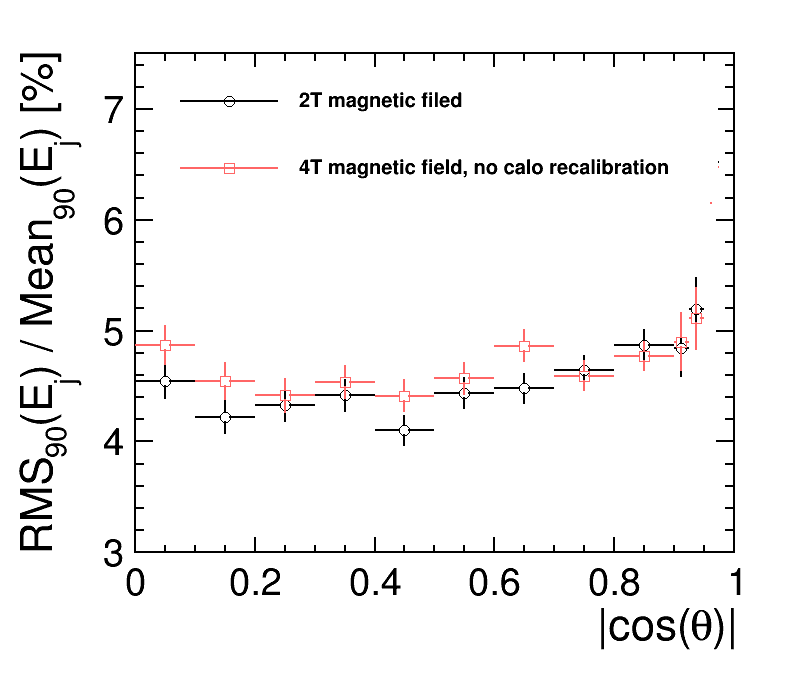
\includegraphics[width=6cm]{jet_energy_res_2Tvs4T_Zuds91.pdf}};
  
 \node[inner sep=0pt] (tmp) at (\xRefPosOne+4.5,\yRefPosOne+0.9)
{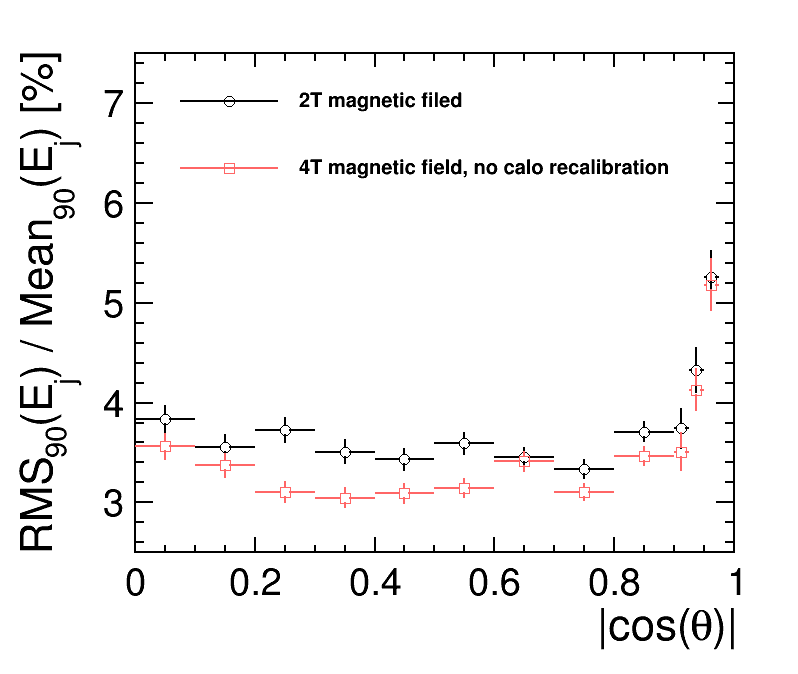
\includegraphics[width=6cm]{jet_energy_res_2Tvs4T_Zuds380.pdf}};

  
  
  
 
 \node  at (\xRefPosOne-0.3,\yRefPosOne-2.8) (box){%
    \begin{minipage}{0.8\textwidth}
      \begin{itemize}
		\item No effect of stronger field at 91 GeV
		\item Better performance at 380 GeV
      \end{itemize}
    \end{minipage}
  };
  
\end{tikzpicture}
\end{frame}
%*****************************************************************************
%*****************************************************************************
\begin{frame}{\large \large New detector model and outlook}
 
 \renewcommand{\yRefPosOne}{0} 
\renewcommand{\xRefPosOne}{5.3}
\renewcommand{\xRefIncrementOne}{5.5}
\begin{tikzpicture}[overlay]

\node [PixelBox] at (\xRefPosOne,\yRefPosOne+1) (box){%
  \begin{minipage}{0.99\textwidth}
  
\begin{itemize}
 \item new FCCee$\_$o1$\_$v03 detector model\\[0.05cm]
 \begin{itemize}
 \item extend ECAL endcap\\[0.1cm]
 \item shrink HCAL ring\\[0.1cm]
 \item reduce magnetic field in barrel yoke from 1.5 T to 1.0 T\\[0.1cm]
 \item fix in HCAL layer layout (no impact on detector performance)\\[0.2cm]
 \end{itemize}
 \item Available in iLCSoft release by April 26
 \end{itemize}


    
  \end{minipage}
};
% \node[fancytitle, right=15pt] at (box.north west) {Outlook};


\node [TRTBox]  at (\xRefPosOne,\yRefPosOne-2) (box){%
  \begin{minipage}{0.99\textwidth}
  
 \begin{itemize}
  \item Update implementation of Bremsstrahlung recovery procedure in MarlinReco/IsolatedLeptonFinder\\[0.1cm]
  \item Background overlay
  \item Software compensation with CLD model
    \end{itemize}
  \end{minipage}
};
\node[fancytitle, right=15pt] at (box.north west) {Outlook};


\end{tikzpicture}
  
\end{frame}
%*****************************************************************************

\end{document}

